\documentclass[a4paper]{article}

\usepackage[utf8x]{inputenc}
\usepackage[british,UKenglish]{babel}
\usepackage{amsmath}
%\usepackage{titlesec}
\usepackage{color}
\usepackage{graphicx}
\usepackage{fancyref}
\usepackage{hyperref}
\usepackage{float}
\usepackage{scrextend}
\usepackage{setspace}
\usepackage{xargs}
\usepackage{multicol}
\usepackage{nameref}
\usepackage[pdftex,dvipsnames]{xcolor}
\usepackage{sectsty}
\usepackage{multicol}
\usepackage{multirow}
\usepackage[procnames]{listings}
\usepackage{appendix}
\usepackage{cite}
\usepackage{pdflscape}

\newcommand\tab[1][1cm]{\hspace*{#1}}
\hypersetup{colorlinks=true, linkcolor=black}
\interfootnotelinepenalty=10000
%\titleformat*{\subsubsection}{\large\bfseries}
%\subsubsectionfont{\large}
%\subsectionfont{\Large}
%\sectionfont{\LARGE}
\definecolor{cleanOrange}{HTML}{D14D00}
\definecolor{cleanYellow}{HTML}{FFFF99}
\definecolor{cleanBlue}{HTML}{3d0099}
%\newcommand{\cleancode}[1]{\begin{addmargin}[3em]{3em}\fcolorbox{cleanOrange}{cleanYellow}{\texttt{\textcolor{cleanOrange}{#1}}}\end{addmargin}}
\newcommand{\cleancode}[1]{\begin{addmargin}[3em]{3em}\texttt{\textcolor{cleanOrange}{#1}}\end{addmargin}}
\newcommand{\cleanstyle}[1]{\text{\textcolor{cleanOrange}{\texttt{#1}}}}


\usepackage[colorinlistoftodos,prependcaption,textsize=footnotesize]{todonotes}
\newcommandx{\commred}[2][1=]{\textcolor{Red}
{\todo[linecolor=red,backgroundcolor=red!25,bordercolor=red,#1]{#2}}}
\newcommandx{\commblue}[2][1=]{\textcolor{Blue}
{\todo[linecolor=blue,backgroundcolor=blue!25,bordercolor=blue,#1]{#2}}}
\newcommandx{\commgreen}[2][1=]{\textcolor{OliveGreen}{\todo[linecolor=OliveGreen,backgroundcolor=OliveGreen!25,bordercolor=OliveGreen,#1]{#2}}}
\newcommandx{\commpurp}[2][1=]{\textcolor{Plum}{\todo[linecolor=Plum,backgroundcolor=Plum!25,bordercolor=Plum,#1]{#2}}}

\def\code#1{{\tt #1}}

\def\note#1{\noindent{\bf [Note: #1]}}

\makeatletter
%% The "\@seccntformat" command is an auxiliary command
%% (see pp. 26f. of 'The LaTeX Companion,' 2nd. ed.)
\def\@seccntformat#1{\@ifundefined{#1@cntformat}%
   {\csname the#1\endcsname\quad}  % default
   {\csname #1@cntformat\endcsname}% enable individual control
}
\let\oldappendix\appendix %% save current definition of \appendix
\renewcommand\appendix{%
    \oldappendix
    \newcommand{\section@cntformat}{\appendixname~\thesection\quad}
}
\makeatother
% "define" Scala
\usepackage[T1]{fontenc}  
\usepackage[scaled=0.82]{beramono}  
\usepackage{microtype} 

\sbox0{\small\ttfamily A}
\edef\mybasewidth{\the\wd0 }

\lstdefinelanguage{scala}{
  morekeywords={abstract,case,catch,class,def,%
    do,else,extends,false,final,finally,%
    for,if,implicit,import,match,mixin,%
    new,null,object,override,package,%
    private,protected,requires,return,sealed,%
    super,this,throw,trait,true,try,%
    type,val,var,while,with,yield},
  sensitive=true,
  morecomment=[l]{//},
  morecomment=[n]{/*}{*/},
  morestring=[b]",
  morestring=[b]',
  morestring=[b]"""
}

\usepackage{color}
\definecolor{dkgreen}{rgb}{0,0.6,0}
\definecolor{gray}{rgb}{0.5,0.5,0.5}
\definecolor{mauve}{rgb}{0.58,0,0.82}

% Default settings for code listings
\lstset{frame=tb,
  language=scala,
  aboveskip=3mm,
  belowskip=3mm,
  showstringspaces=false,
  columns=fixed, % basewidth=\mybasewidth,
  basicstyle={\small\ttfamily},
  numbers=none,
  numberstyle=\footnotesize\color{gray},
  % identifierstyle=\color{red},
  keywordstyle=\color{blue},
  commentstyle=\color{dkgreen},
  stringstyle=\color{mauve},
  frame=single,
  breaklines=true,
  breakatwhitespace=true,
  procnamekeys={def, val, var, class, trait, object, extends},
  procnamestyle=\ttfamily\color{red},
  tabsize=2
}

\lstnewenvironment{scala}[1][]
{\lstset{language=scala,#1}}
{}
\lstnewenvironment{cpp}[1][]
{\lstset{language=C++,#1}}
{}
\lstnewenvironment{bash}[1][]
{\lstset{language=bash,#1}}
{}
\lstnewenvironment{verilog}[1][]
{\lstset{language=verilog,#1}}
{}



\lstset{frame=, basicstyle={\footnotesize\ttfamily}}



\graphicspath{ {images/} }

%-----------------------------------------BEGIN DOC----------------------------------------

\begin{document}

\title{{\Huge ercesiMIPS Lab Report{\large\linebreak\\}}{\Large Lab1 Single Cyclic CPU with 7-9(11) MIPS Instructions\linebreak\linebreak}}
%please write your name, Student #, and Class # in Authors, student ID, and class # respectively
\author{\\Name: Firstname Lastename\\
StudentID: xxxxxx\\
Class\#: xxxxx\\\\
CS 11007 Computer Organization and Architecture\\
(Spring, 2017)\\\\
Northwestern Polytechnical University, China\\
Faculty of Computer Science\\
ERCESI}
\date{\today}
\maketitle
\newpage

%-----------------------------------------ABSTRACT-------------------------------------
\begin{center}
{\large\bf{Abstract\\}}
\end{center}
Please enter the abstract here, just summary your lab works.
\newpage
%-----------------------------------------ABSTRACT-------------------------------------
\begin{center}
{\large\bf{Copyright Statement\\}}
\end{center}
The copyright law of China governs the making of photocopies or other reproductions of copyrighted material. All right reserved. No portion of this document may be photocopied and reproduced without written permission from ERCESI (NWPU) except by a reviewer who may quote brief passages in connection with a citation. \\\\
ERCESI Reserves the right to refuse a copying order if, in its judgment, fulfillment of the order would involve violation of copyright law.If a user makes a request for, or later uses, a photocopy or reproduction without a writtern permission from ERCESI, the user may be liable for copyright infringement.\newpage
%-----------------------------------------CONTENT-------------------------------------
\tableofcontents\label{c}
\newpage

%------------------------------------------TEXT--------------------------------------------

%----------------------------------------OVERVIEW-----------------------------------------

\section{Overview} \label{overview}%------------------------------
The structure of Single cyclic MIPS CPU has been introduced in CS 11007 class lecture.
\begin{itemize}
	\item{\textbf{Supported Instructions} includes \emph{sub, add, or, ori, lw, sw, lst, beq, j}, or adding \emph{addi, and, andi} for better programming experience in assembly. All these instructions can be supported without exception detecting (overflow detecting)}
    \item{\textbf{All instructions work in one cycle.} For the very beginning stage, Single Cyclic CPU model is a great example to explain how CPU works.}
    \item{\textbf{Consisted of Data Path, Control Unit and Memory Unit.} To illustrate the typical systematic idea of computer, we recommend you design your first CPU with two separated modules, CPath and DPath, in such coding style, both blocks can also be easily verified separately. Additionally, if more complement MIPS ISA is chosen, this structure will be high efficient to be extended.}
    \item{\textbf{Chisel3 is also recommended.} Chisel is a powerful structural hardware description language, with more efficient expression for block, operation, and IO bundles compared with Verilog. However, the most significant feature of Chisel is that it can express the structure of system without detailed circuits coding. Further more, we prefer Chisel3 instead of Chisel2, which relies on verilator for verilog simulations instead of Synopsys vcs. The difference between these tow versions can be referenced here: \url{https://github.com/ucb-bar/chisel3/wiki/Chisel3-vs-Chisel2}.}
\end{itemize}

%----------------------------------SYSTEM DESIGN------------------------------------------

\newpage
\section{System Design} \label{sysdes}%------------------------------
\subsection{System Overview}\label{sub:sysover}
Please describe your CPU system design here, Figures are recommended for detailed illustration and add the figure using latex could be reference the insertion of Fig. \ref{fig:singleblock}. 
\begin{figure}[ht]
 \centering
 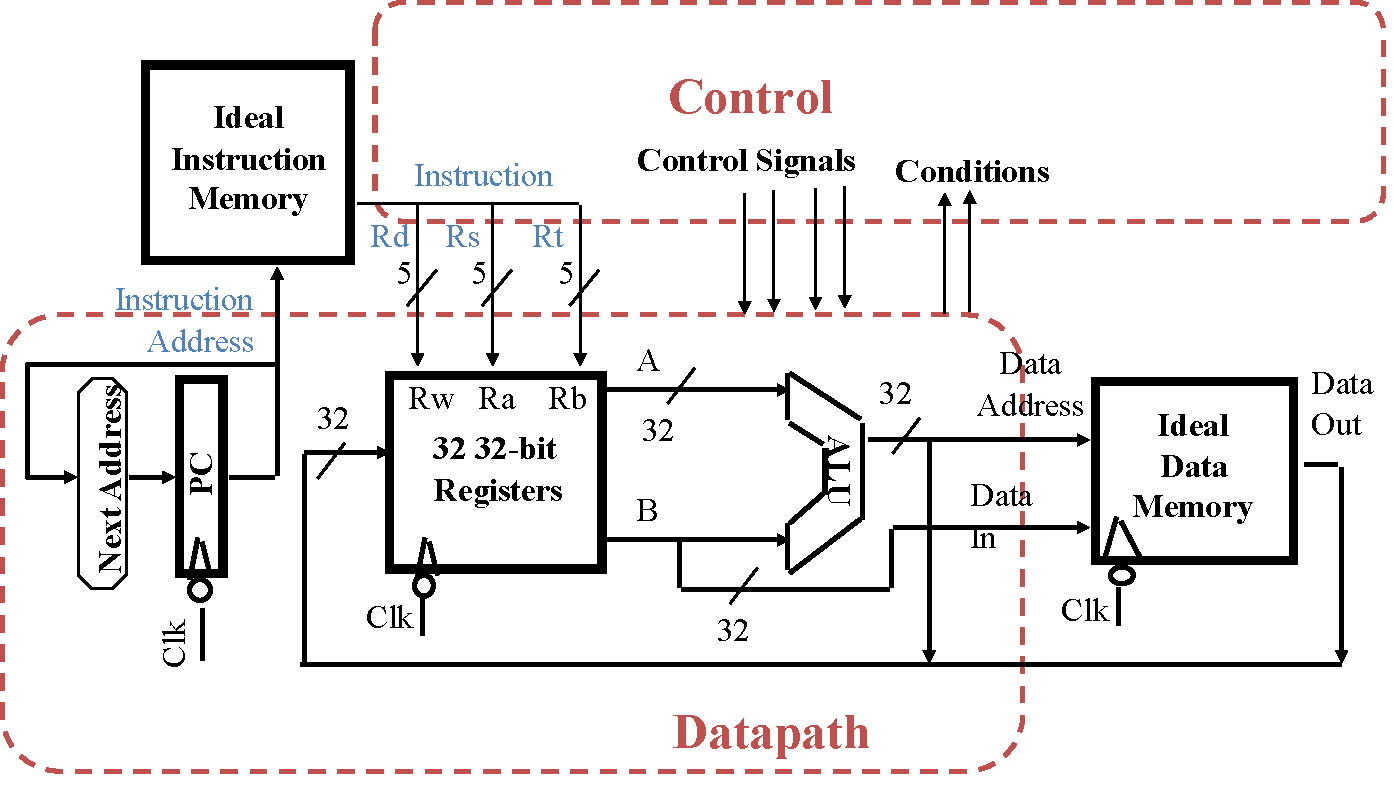
\includegraphics[height=5cm]{images/l1sys.pdf}
 \caption{Single Cyclic CPU Block Diagram}
 \label{fig:singleblock}
\end{figure}
If you need cite a reference like this \cite{Erdos01}, and a sample bibliography item is attached at the end.
\subsection{Interface Definition}\label{sub:Interface}
In this section, the interfaces among the blocks of top level should be described in details. Tables can be used in latex as this. Table \ref{tab:signaldef}

\begin{table}[htp]
\caption{Signals Definition for Test Mode}\label{tab:signaldef}
\begin{center}
	\begin{tabular}{|l|l|l|p{6cm}|}
	\hline
	\textbf{Signal Name} & \textbf{Direction} & \textbf{Width} & \textbf{Function}\\ \hline \hline
	boot			& Input 	& 1-bit	& Trigger the boot test mode, 
									  set to 0 in CPU regular process mode\\ \hline
	test\_im\_wr 	& Input	& 1-bit	& Instruction memory write enable in test mode,set to 0 in 	
								  CPU regular process mode. In test mode, it will be set to 1 when if writing instructions to imem, otherwise it is set to 0.\\ \hline
	test\_im\_re 	& Input & 1-bit & Instruction memory read enable in test mode,set to 0 in 	
								  CPU regular process mode. In test mode, it will be set to 1 when if reading instructions out, otherwise it is set to 0. \\ \hline
	test\_im\_addr 	& Input & 32-bit& Instruction memory address\\ \hline
	test\_im\_in 	& Input & 32-bit& Instruction memory data input for test mode. \\ \hline
	test\_im\_out 	& Output& 32-bit& Instruction memory data output for test mode. \\ \hline
	test\_dm\_wr 	& Input	& 1-bit	& Data memory write enable in test mode,set to 0 in 	
								  CPU regular process mode. In test mode, it will be set to 1 when if writing data to dmem, otherwise it is set to 0.\\ \hline
	test\_dm\_re 	& Input & 1-bit & Data memory read enable in test mode,set to 0 in 	
								  CPU regular process mode. In test mode, it will be set to 1 when if reading data out, otherwise it is set to 0.\\ \hline
	test\_dm\_addr 	& Input & 32-bit& Data memory address\\ \hline
	test\_dm\_in 	& Input & 32-bit& Data memory input for test mode. \\ \hline
	test\_dm\_out 	& Output& 32-bit& Data memory output for test mode. \\ \hline
	valid			& Output& 1-bit & If CPU stopped or any exception happens, valid signal is set to 0.\\ 
	\hline
	\end{tabular}
\end{center}
\end{table}

\subsection{(Sequential) Logic of Interface}\label{sub:logicinter}
Please define the logic of interfaces of your top level. Figures and tables also will be helpful for expressing ideas in academic style.
% -----------------------------------BLOCKS DESIGN----------------------------------------
\section{Blocks Design}
This section is for detailed introduction of block function, interface definition, logic implementation (FSM design), etc. for every single block.
\subsection{ALU}\label{sub:alu}
\subsubsection{Function}
\subsubsection{Interface Definition}
\subsubsection{Logic Design}

\subsection{Control Unit}\label{sub:ctl}
\subsubsection{Function}
\subsubsection{Interface Definition}
\subsubsection{Logic Design}

\subsection{Data Path}\label{sub:dat}
\subsubsection{Function}
\subsubsection{Interface Definition}
\subsubsection{Logic Design}

%add more subsections for other block in you CPU design.

\section{Lab Records}\label{labrec}
The whole lab process, all design events, problems and relevant solutions are described here. Name your Subsections according to demand.

% -----------------------------------Appendix----------------------------------------
\appendix
%\renewcommand{\appendixname}{Appendix~\Alph{section}}
\section{Code}\label{sub:app.code}
Please add your code with Scala syntax highlight support like below.This is app \ref{sub:app.code}
\begin{scala}
class TopIO extends Bundle() {
	val boot = Input(Bool()) 
// imem and dmem interface for Tests
	val test_im_wr		= Input(Bool())
	val test_im_rd 		= Input(Bool())
	val test_im_addr 	= Input(UInt(32.W))
	val test_im_in 		= Input(UInt(32.W))
	val test_im_out 	= Output(UInt(32.W))

	val test_dm_wr		= Input(Bool())
	val test_dm_rd 		= Input(Bool())
	val test_dm_addr 	= Input(UInt(32.W))
	val test_dm_in 		= Input(UInt(32.W))
	val test_dm_out 	= Output(UInt(32.W))

	val valid			= Output(Bool())
}
class Top extends Module() {
	val io 		= IO(new TopIO())//in chisel3, io must be wrapped in IO(...) 
	//...
	when (io.boot & io.test_im_wr){
		imm(io.test_im_addr) := io.test_im_in
		} .elsewhen (io.boot & io.test_dm_wr){
		// please finish it
		} //...
}
\end{scala}
\newpage
% -----------------------------------REFERENCE----------------------------------------
\begin{thebibliography}{9}
\bibitem{Erdos01} P. Erd\H os, \emph{A selection of problems and
results in combinatorics}, Recent trends in combinatorics (Matrahaza,
1995), Cambridge Univ. Press, Cambridge, 2001, pp. 1--6.
\end{thebibliography}
\end{document}

